\chapter{Method}
% \thispagestyle{fancy}
% FIXME -- change from cross model to vae-gan

The method used in the thesis is the \ac{vae}-\ac{gan} hybrid discussed in \ref{subsec:vaeganhybrid}. Except that the Similarly function used is \ac{l1} loss and not the \ac{gan} similarity metric \ref{eqn:gan_similarity}. The details are further described in the section.
%TODO -- Add architecutre image here

\section{Architecture}

The \ac{vae}-\ac{gan} hybrid architecture is illustrated in fig. \ref{fig:method_arch}

\subsection{VAE} 
Similar to the \ac{vae}-\ac{gan} described in \ref{subsec:vaeganhybrid}, the proposed architecture consists of an encoder, decoder and a discriminator. The encoder takes the 2D pose as input and encodes it in a latent space. The decoder samples this encoding using the reparametrization trick and outputs a 3D pose. Following the best practices from \cite{soumith2017wasserstein}, the decoder which is also the generator is made to output 3D poses with values from [-1,1] and Tanh activation is used at the output of the decoder. As described in \ref{chap:data}, the 3D pose is modelled to be of unit length from root to head. However the lower half of the body could be higher than that. To handle this, the output is multiplied by 2 to cover the true dimensions of the lower half.

\begin{figure}[!h]
    \centering
    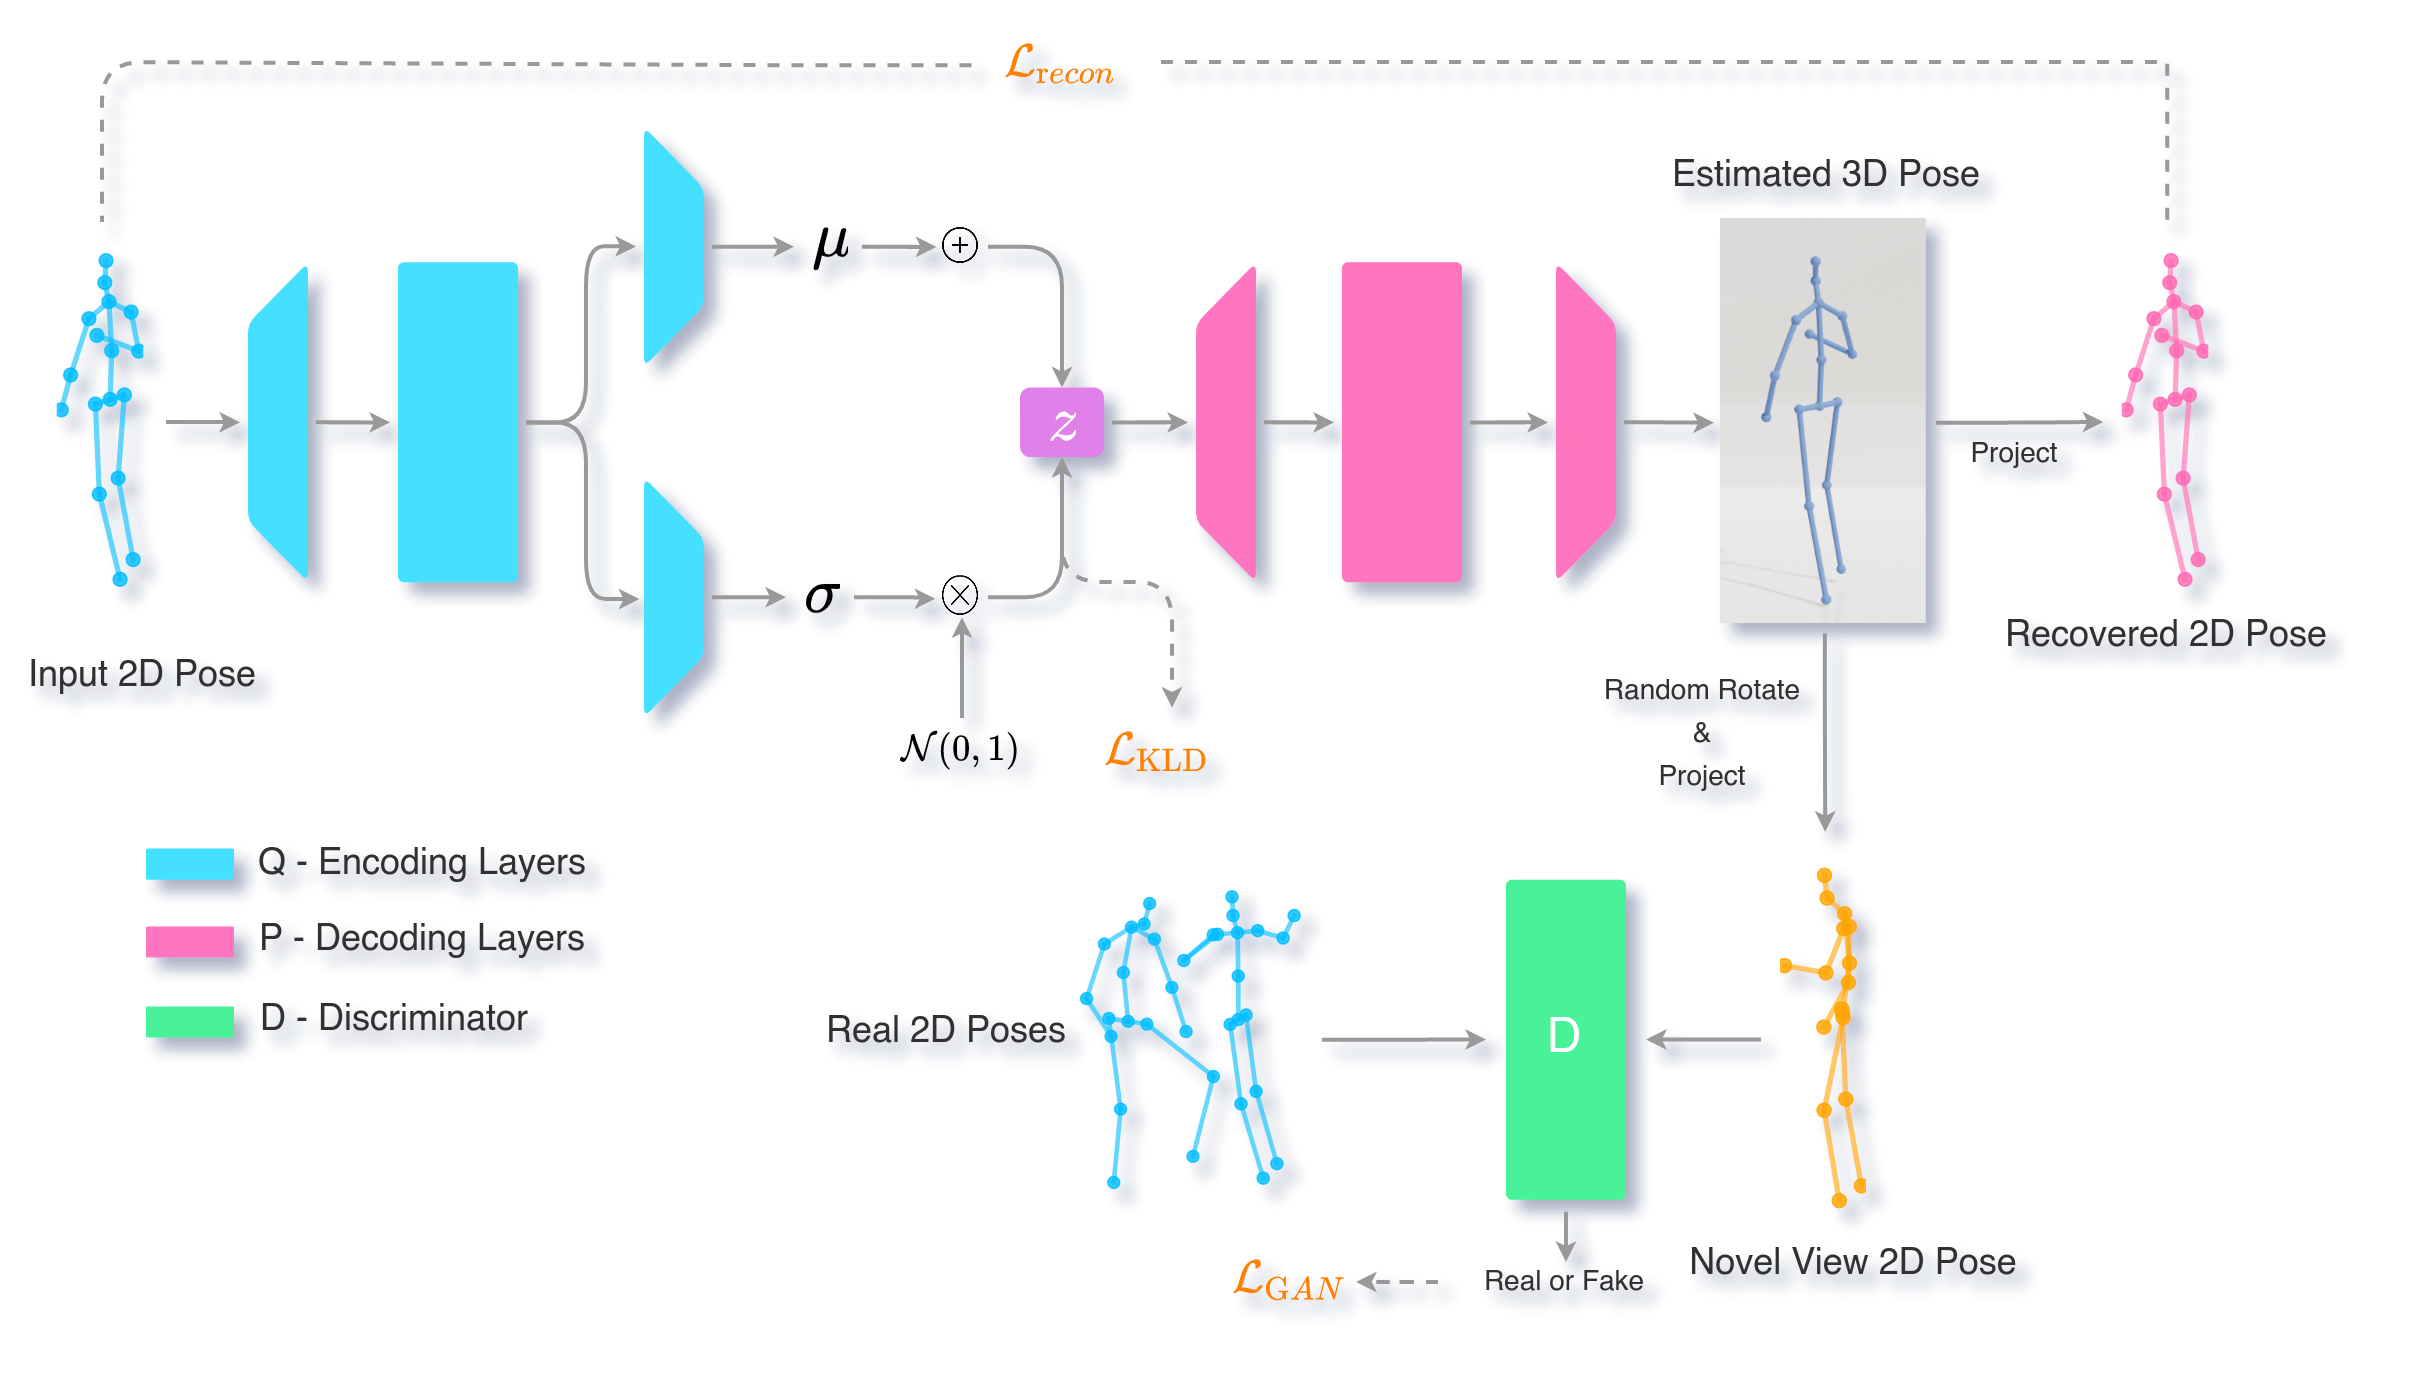
\includegraphics[scale=0.2]{figures/arch/method_arch.png}
    \caption{Illustration of the architecutre and loss flow in the proposed approach. }
    \label{fig:method_arch}
\end{figure}


The encoder consists of an upsampling layer that makes the $2 \cdot j$ dimensional input to match the number of hidden neurons of the encoding module. Where $j$ is the number of joints, here 16. The encoding module is made of $n$ residual block composed of 2 \ac{fc} layers following the related works, so as to allow comparision. Where $n$ is usually 1 or 2. The enoding block is followed by 2 \ac{fc} layers that down sample the hidden representation to match the latent space dimension. The output of the two downsampling layers represent the mean and variance of the embedding in the latent space. All the layers use \ac{relu} activation unless specified otherwise. The decoder mimics the encoder with an upsampling layer, a decoding module and a downsampling layer to output 3D pose of dimension $3 \cdot j$.

\subsection{Discriminator}%FIXME -- \subsection{Image \ac{vae}}
The discriminator following the related works also mimics the generator and takes 2D poses as input and predicts binary labels of real or false. The sigmoid activation function is used at the output layer of the discriminator.


\section{Training Scheme}
The training scheme is similar to the standard \ac{vae} and \ac{vae}-\ac{gan} introduced in \ref{sec:Preliminary}. The discriminator is trained first for a few steps before training the \ac{vae}. First, the \ac{vae} takes the 2D pose as input and predicts the 3D pose. This predicted 3D pose is first reprojected to 2D to train the \ac{vae} and then randomly rotated and reprojected to a novel 2D view. This novel 2D is used as the fake samples to train the discriminator. As \ac{vae} learns to improve the reprojected 2D pose, it will eventually be very close to the real samples. Using these as the fake examples will not be very useful as the decoder is do the same job. Training the discriminator on randomly rotated and reprojected 2D novel view would encorage the decoder to generate pose that not only agree with the input 2D pose but ensure that the other view of the 3D is also indistingusable from the variations found in the data by fooling the discriminator. This two view supervision leads to better 3D pose generations.
% \section{Bag of tricks} % TODO -- add tricks to make it work here or in work? -- it should be here
% \lipsum[1-10] %FIXME

\section{Evaluation Metrics} % FIXME
3D \ac{hpe} and Human3.6M in particular is mainly evaluated by \ac{mpjpe} metric. MPJPE as it literally abbreviates, is the mean of the position estimate for all the joints of a pose. Where per-joint position estimate is nothing but the euclidian distance (usually measured in mm) between the predicted joint to its ground truth.
